\documentclass[10pt,compress,mathserif]{beamer}
\usetheme{Berkeley}
% Few theme names Berkeley Copenhagen Dresden


\usepackage{amsmath,minibox,amssymb,amsfonts,amsthm,graphicx,color,multirow,array,tikz,hyperref}
\usetikzlibrary{arrows,snakes,backgrounds,patterns,matrix,shapes,fit,calc,shadows, positioning}

\setbeamertemplate{navigation symbols}{} % This is just to get rid of the extra fazool symbols
\setbeamerfont{caption}{size=\footnotesize}

\title[]{Control Systems Project}
\author[]{Waseem Ullah Khan\\ Section A DCSE \\ UET Peshawar.}
\rightskip=0pt plus 0pt
\boldmath

\begin{document}

\begin{frame}    \titlepage \end{frame}



% First slide
\section{Introduction}
\begin{frame}{Introduction to Project}
\noindent Perform the following for E2.13 at Page 82:\\ \vskip10pt
a. Obtain state-space representation for the system (without obtaining any transfer function). \\ \vskip10pt
b. Choose the output matrix as you like (except identity matrix - and make the system observable). \\ \vskip10pt
c. Check the stability of the system using all methods that you know.\\ \vskip10pt
d. Compute the controllability and observability for the system. If the system is controllable, place the controller poles at (-3, -5) and observer poles at a location which is faster than the controller poles.\\ \vskip10pt
e. Simulate the system using observer based feedback controller and show all the responses.

\end{frame}



% Second Slide
\section{Solution}
\begin{frame}{State-space Representation of the System}
The state-space representation of the system can be written as follows:
\begin{equation}
\begin{bmatrix} \dot{x_1}\\  \dot{x_2} \end{bmatrix}
= \begin{bmatrix}
1 & 2 \\
3 & 4  \end{bmatrix}
\begin{bmatrix} x_1\\  x_2 \end{bmatrix} +
\begin{bmatrix}
5 & 6 \\
13 & 7  \end{bmatrix}
\begin{bmatrix} u_1\\  u_2 \end{bmatrix}
\end{equation}

\begin{equation}
y=\begin{bmatrix}
1 \\ -0.3
\end{bmatrix}x
\end{equation}

\end{frame}


\section{Stability Analysis}
\begin{frame}{Stability Analysis of the System}
The eigen values of the system are:
\begin{equation} \lambda_1 = 3,  \lambda_2 = -20 \end{equation} \vskip10pt

The poles of the system are:
\begin{equation} p_1 = 3,  p_2 = -20 \end{equation} \vskip10pt

\end{frame}

\begin{frame}{Stability Analysis of the System}
Routh-Hurwitz table is shown below
\begin{table}[h] \begin{center}
\begin{tabular}{|l|c|l|} \hline
$s^3$  & 1 & 31 \\ \hline
$s^2$  & 10 & 31 \\ \hline
$s^1$  & $-\frac{1}{10}\times\begin{vmatrix} 1 & 31\\ 10 & 31 \end{vmatrix}=27.9$ & 0 \\
$s^0$  & $-\frac{1}{27.9}\times\begin{vmatrix} 10 & 31\\ 27.9 & 0.1 \end{vmatrix}=31$ & 0 \\ \hline
\end{tabular} \end{center}
\end{table}

As there are no sign changes in the first column, the system is stable.


\end{frame}


\begin{frame}{Stability Analysis of the System}
The step response of the system is:
\begin{figure}[h!]
\centering
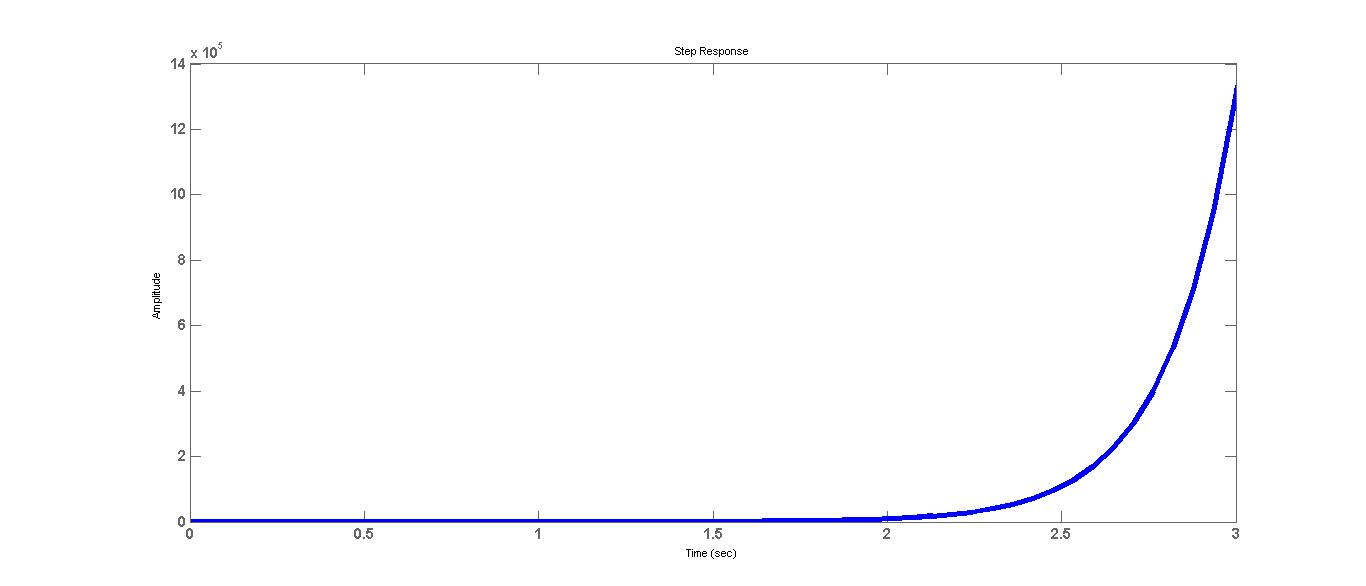
\includegraphics[scale=0.2]{Step_Res.jpg}
\caption{Plot of step response.}
\end{figure}
\end{frame}





\section{Controllability}
\begin{frame}{Controllability Analysis}
\end{frame}


\section{Observability}
\begin{frame}{Observability Analysis}
\end{frame}


\section{Controller Design}
\begin{frame}{Controller Design}
\end{frame}


\section{Results}
\begin{frame}{Results}
Put results without controller and with controller \\ \vskip10pt
Compute steady state errors and show those errors before controller design, after controller design, and after tracking controller design \\ \vskip10pt
Verify the steady state errors from Matlab or Simulink by step response and ramp response (be careful with the magnitude of step input and ramp input - it should be the same as your project question).

\end{frame}



\end{document} 